\documentclass[tikz,border=2pt]{standalone}
\usepackage{amsmath}
\usepackage{pgfplots}
\pgfplotsset{compat=1.18}

\begin{document}
% Restricting f to the subset S keeps the same rule but only over S: the graph of f|_S is the
% highlighted piece of the graph of f.
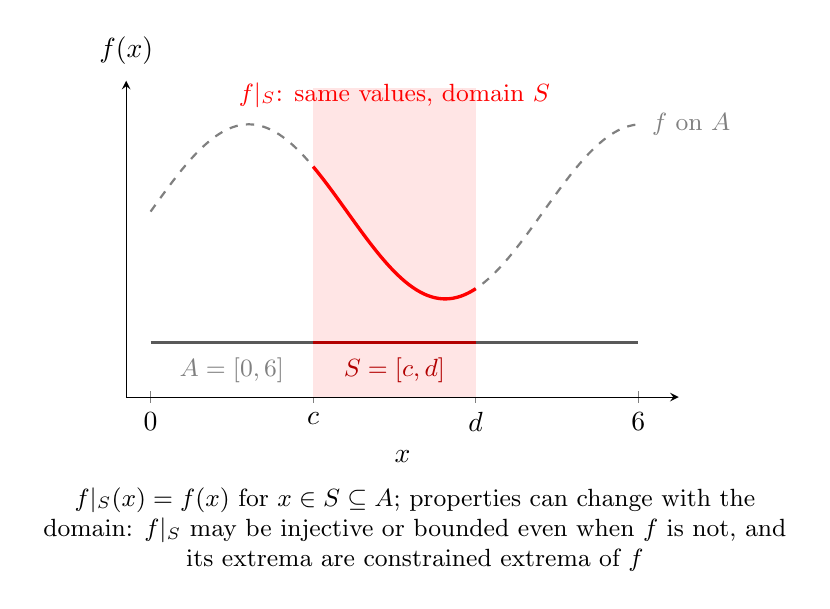
\begin{tikzpicture}
	\begin{axis}[
		axis lines=left, xmin=-0.3, xmax=6.5, ymin=-0.75, ymax=3.6,
		xtick={0,2,4,6}, xticklabels={$0$,$c$,$d$,$6$}, ytick=\empty,
		xlabel={$x$}, ylabel={$f(x)$}, ylabel style={rotate=-90, anchor=south, at={(axis description cs:0,1.02)}},
		samples=160, smooth, width=8.6cm, height=5.6cm, clip=false
		]
		\fill[red!10] (axis cs:2,-0.75) rectangle (axis cs:4,3.5);
		\addplot[gray, thick, dashed, domain=0:6] {1.8+1.2*sin(deg(1.3*x))};
		\addplot[red, very thick, domain=2:4] {1.8+1.2*sin(deg(1.3*x))};
		\draw[gray!70!black, very thick] (axis cs:0,0) -- (axis cs:6,0);
		\draw[red!70!black, very thick] (axis cs:2,0) -- (axis cs:4,0);
		\node[gray, font=\small, anchor=north] at (axis cs:1.0,-0.08) {$A=[0,6]$};
		\node[red!70!black, font=\small, anchor=north] at (axis cs:3,-0.08) {$S=[c,d]$};
		\node[gray, anchor=west, font=\small] at (axis cs:6.05,3.0) {$f$ on $A$};
		\node[red, anchor=south, font=\small] at (axis cs:3,3.1) {$f|_S$: same values, domain $S$};
	\end{axis}
	\node[anchor=north, font=\small, align=flush center, text width=9.6cm] at ([yshift=-2pt]current axis.outer south) {$f|_S(x)=f(x)$ for $x\in S\subseteq A$; properties can change with the domain: $f|_S$ may be injective or bounded even when $f$ is not, and its extrema are constrained extrema of $f$};
\end{tikzpicture}
\end{document}
